\documentclass{article}

\usepackage[T1]{fontenc}
\usepackage[utf8]{inputenc}

\usepackage{relsize}
\usepackage{lmodern}
\usepackage[babel]{microtype}
\usepackage{comment}

\clubpenalty = 10000
\widowpenalty = 10000

\usepackage{listings}

% In-text code style (breakable and unbreakable)
\newcommand{\brcode}[1]{\textsf{#1}}
\newcommand{\code}[1]{\mbox{\brcode{#1}}}

\lstloadlanguages{Java}
\lstloadlanguages{JVMIS}

\lstset{
  columns=fullflexible,
  mathescape=true,
  escapechar={~},
  basicstyle=\relsize{0}\ttfamily,
  showstringspaces=false,
}

\usepackage{hyperref}
\usepackage[all]{hypcap}

\hypersetup{
  unicode = true,
  colorlinks = true,
  linkcolor = black,
  anchorcolor = black,
  citecolor = black,
  urlcolor = black,
  % Don't use guessable names for links; required for subfloat compatibility.
  hypertexnames = false,
}

\urlstyle{sf}

\usepackage{graphicx}

\sloppy

\begin{document}

\title{Introduction to Instrumentation with DiSL}

\maketitle

\section{Introduction}

DiSL is a domain-specific language for Java bytecode instrumentation.
DiSL is inspired by AOP, but in contrast to mainstream AOP languages, it features an open join point model where any region of bytecodes can be selected as a join point (i.e., code location to be instrumented).
DiSL reconciles high-level language constructs resulting in concise instrumentations, high expressiveness, and efficiency of the inserted instrumentation code.
Thanks to the pointcut/advice model adopted by DiSL, instrumentations are similarly compact as aspects written in AspectJ.
However, in contrast to AspectJ, DiSL does not restrict the code locations that can be instrumented, and the code generated by DiSL avoids expensive operations (such as object allocations that are not visible to the programmer).
Furthermore, DiSL supports instrumentations with complete bytecode coverage out-of-the-box and avoids structural modifications of classes that would be visible through reflection and could break the instrumented code.


\section{DiSL by Example}\label{sec:DiSL}

A common example of a dynamic program analysis tool is a method execution time profiler, which usually instruments the method entry and exit join~points and introduces storage for timestamps.
We describe the main features of DiSL by gradually developing the instrumentation for such a profiler.
The same instrumentation is also available on the DiSL home page\footnote{\url{http://disl.ow2.org}} among the examples.
For step-by-step instructions on how to run the examples, please refer to Appendix~\ref{sec:Setup}.

While running DiSL, you can encounter issues like crashes or assertion violations in JVM.
This is not directly problem of DiSL but rather limitation of JVM itself.
For more information, please refer to Appendix~\ref{sec:Crashes}.


\subsection{Method Execution Time Profiler}

% The structure of each step should be roughly:
% 1. What profiler features we develop now.
% 2. What DiSL features are used for that.
% 3. Code explanation.
% 4. Comments.

In the first version of our execution time profiler, we simply print the entry and exit times for each method execution as it happens.
For that, we need to insert instrumentation at the method entry and method exit join~points.

Each DiSL instrumentation is defined through methods declared in standard Java classes.
Each method---called {\em snippet} in DiSL terminology---is annotated so as to specify the join~points where the code of the snippet shall be inlined.\footnote{The name of the method is not constrained and can be arbitrarily chosen by the programmer.}
The profiler instrumentation code on Figure~\ref{fig:instr-prof-simple-prof} uses two such snippets, the first one prints the entry time, the second one the exit time.

\begin{figure}[h!]
\smaller
\begin{lstlisting}[language=Java]
public class SimpleProfiler {

  @Before(marker=BodyMarker.class)
  static void onMethodEntry() {
    System.out.println("Method entry " + System.nanoTime());
  }

  @After(marker=BodyMarker.class)
  static void onMethodExit() {
    System.out.println("Method exit " + System.nanoTime());
  }
}
\end{lstlisting}
%\vspace{-6mm}
\caption{Instrumenting method entry and exit}
\label{fig:instr-prof-simple-prof}
\end{figure}

The code uses two annotations to direct inlining.
The \code{@Before} annotation requests the snippet to be inlined before each marked bytecode region (representing a join~point); the use of the \code{@After} annotation places the second snippet after (both normal and abnormal) exit of each marked region.
The regions themselves are specified with the \code{marker} parameter of the annotation.
In our example, \code{BodyMarker} marks the whole method (or constructor) body.
The resulting instrumentation thus prints a timestamp upon method entry and exit.

\medskip

Instead of printing the entry and exit times, we may want to print the elapsed wall-clock time from the method entry to the method exit.
The elapsed time can be computed in the after snippet, but to perform the computation, the timestamp of method entry has to be passed from the before snippet to the after snippet.

In traditional AOP languages, which do not support efficient data exchange between advices, this situation would be handled using a local variable within the around advice.
In contrast, an instrumentation framework such as DiSL has no need for the usual form of the around advice, which lets the advice code decide whether to skip or proceed with the method invocation.
DiSL therefore only supports inlining snippets before and after a particular join~point, together with a way for the snippets inlined into the same method to exchange data using \emph{synthetic local variables}, as illustrated on Figure~\ref{fig:instr-prof-time}.

\begin{figure}[h!]
\smaller
\begin{lstlisting}[language=Java]
public class SimpleProfiler {

  @SyntheticLocal
  static long entryTime;

  @Before(marker=BodyMarker.class)
  static void onMethodEntry() {
    entryTime = System.nanoTime();
  }

  @After(marker=BodyMarker.class)
  static void onMethodExit() {
    System.out.println("Method duration " + (System.nanoTime() - entryTime));
  }
}
\end{lstlisting}
%\vspace{-6mm}
\caption{Passing data between snippets using a synthetic local variable}
\label{fig:instr-prof-time}
\end{figure}

Synthetic local variables are static fields annotated as \code{@SyntheticLocal}.
The variables have the scope of a method invocation and can be accessed by all snippets that are inlined in the method; that is, they become local variables.
Synthetic local variables are initialized to the default value of their declared type (e.g., \code{0}, \code{false}, \code{null}).

\medskip

Next, we extend the output of our profiler to include the name of each profiled method.
In DiSL, the information about the instrumented class, method, and bytecode region can be obtained through dedicated \emph{static context interfaces}.
In this case, we are interested in the \code{MethodStaticContext} interface, which provides the method name, signature, modifiers and other static data about the intercepted method and its enclosing class.
Figure~\ref{fig:instr-prof-name} refines the after snippet of Figure~\ref{fig:instr-prof-time} to access the fully qualified name of the instrumented method.

\begin{figure}[h!]
\smaller
\begin{lstlisting}[language=Java]
@After(marker=BodyMarker.class)
static void onMethodExit(MethodStaticContext msc) {
  System.out.println(msc.thisMethodFullName() + " duration "
    + (System.nanoTime() - entryTime));
}
\end{lstlisting}
%\vspace{-6mm}
\caption{Accessing the method name through static context}
\label{fig:instr-prof-name}
\end{figure}

Static context interfaces provide information that is already available at the instrumentation time.
When inlining the snippets, DiSL therefore replaces the calls to these interfaces with the corresponding static context information, thus improving the efficiency of the resulting tools.

DiSL provides a set of commonly used static context interfaces, which can be declared as arguments to the snippets in any order.
The DiSL programmer may also define custom static context interfaces to perform additional static analysis at instrumentation time or to access information not directly provided by DiSL.


\subsection{Adding Stack Trace}

Sometimes knowing the name of the profiled method is not enough.
We may also want to know the context in which the method was called.
Such context is provided by the stack trace of the profiled method.

There are several ways to obtain the stack trace information in Java, such as calling the \code{getStackTrace()} method from \code{java.lang.Thread}, but frequent calls to this method may be expensive.
Our example therefore obtains the stack trace using instrumentation.
Figure~\ref{fig:instr-prof-cs} shows two additional snippets that maintain the call stack information in a shadow call stack.
Upon method entry, the method name is pushed onto the shadow call stack.
Upon method exit, the method name is popped off the shadow call stack.

\begin{figure}[h!]
\smaller
\begin{lstlisting}[language=Java]
@ThreadLocal
static Stack<String> callStack;

@Before(marker=BodyMarker.class, order=1000)
static void pushOnMethodEntry(MethodStaticContext msc) {
  if (callStack == null) { callStack = new Stack<String>(); }
  callStack.push(msc.thisMethodFullName());
}

@After(marker=BodyMarker.class, order=1000)
static void popOnMethodExit() {
  callStack.pop();
}
\end{lstlisting}
%\vspace{-6mm}
\caption{Reifying a thread-specific call stack using dedicated snippets}
\label{fig:instr-prof-cs}
\end{figure}

Each thread maintains a separate shadow call stack, referenced by the thread-local variable~\code{callStack}.\footnote{DiSL offers a particularly efficient implementation of thread-local variables with the \code{@ThreadLocal} annotation.}
In our example, \code{callStack} is initialized for each thread in the before snippet.
The thread-local shadow call stack can be accessed from all snippets through the \code{callStack} variable; for example, it could be included in the profiler output.

To make sure all snippets observe the shadow call stack in a consistent state, the two snippets that maintain the shadow call stack have to be inserted in a correct order relative to the other snippets.
DiSL allows the programmer to specify the order in which snippets matching the same join~point should be inlined using the \code{order} integer parameter in the snippet annotation.
The smaller this number, the closer to the join~point the snippet is inlined.
In our profiler, the time measurement snippets and the shadow call stack snippets match the same join~points (method entry, resp. method exit).
We assign a higher order value (1000) to the call stack reification snippets and keep the lower default order value (100) of the snippets for time measurement.\footnote{If snippet ordering is used, it is recommended to override the value in all snippets for improved readability.}
Consequently, the callee name is pushed onto the shadow call stack before the entry time is measured, and the exit time is measured before the callee name is popped off the stack.


\subsection{Profiling Object Instances}

Our next extension addresses situations where the dependency of the method execution time on the identity of the called object instance is of interest.
Figure~\ref{fig:instr-prof-identity} refines the after snippet of Figure~\ref{fig:instr-prof-time} by computing the identity hash code of the object instance on which the intercepted method has been called.

\begin{figure}[h!]
\smaller
\begin{lstlisting}[language=Java]
@After(marker=BodyMarker.class)
static void onMethodExit(MethodStaticContext msc, DynamicContext dc) {
  int identityHC = System.identityHashCode(dc.getThis());
  ...
}
\end{lstlisting}
%\vspace{-6mm}
\caption{Accessing dynamic context information in a snippet}
\label{fig:instr-prof-identity}
\end{figure}

The snippet uses the \code{DynamicContext} \emph{dynamic context interface} to get a reference to the current object instance.
Similar to the static context interfaces, the dynamic context interfaces are also exposed to the snippets as method arguments.
Unlike the static context information, which is resolved at instrumentation time, calls to the dynamic context interface are replaced with code that obtains the required dynamic information at runtime.
Besides the object reference used in the example, DiSL provides access to other dynamic context information including the local variables, the method arguments, and the values on the operand stack.


\subsection{Selecting Profiled Methods}

Often, it is useful to restrict the instrumentation to certain methods.
For example, we may want to profile only the execution of methods that contain loops, because such methods are likely to contribute more to the overall execution time.

DiSL allows programmers to restrict the instrumentation scope using the \emph{guard} construct.
A guard is a user-defined class whose one method carries the \code{@GuardMethod} annotation.
This method determines whether a snippet matching a particular join~point is inlined.
Figure~\ref{fig:instr-guard} shows the signature of a guard restricting the instrumentation only to methods containing loops.
The body of the \code{methodContainsLoop()} guard method, not shown here, would implement the detection of a loop in a method.
A loop detector based on control flow analysis is included as part of DiSL.

\begin{figure}[h!]
\smaller
\begin{lstlisting}[language=Java]
public class MethodsContainingLoop {

  @GuardMethod
  public static boolean methodContainsLoop() {
    ... // Loop detection based on control flow analysis
  }
}
\end{lstlisting}
%\vspace{-6mm}
\caption{Skeleton of a guard for selecting only methods containing a loop}
\label{fig:instr-guard}
\end{figure}

The loop guard is associated with a snippet using the \code{guard} annotation parameter, as illustrated in Figure~\ref{fig:instr-prof-loopguard}.
Note that the loop guard is not used in the shadow call stack snippets.
We want to maintain complete stack trace information without omitting the methods that do not contain loops.

\begin{figure}[h!]
\smaller
\begin{lstlisting}[language=Java]
@Before(marker=BodyMarker.class, guard=MethodsContainingLoop.class)
static void onMethodEntry() { ... }

@After(marker=BodyMarker.class, guard=MethodsContainingLoop.class)
static void onMethodExit(...) { ... }
\end{lstlisting}
%\vspace{-5mm}
\caption{Applying time measurement snippets only in methods containing a loop}
\label{fig:instr-prof-loopguard}
\end{figure}


\section{Advanced DiSL Features}\label{sec:Advanced}

% Subsection names originally reflected what extension to the profiler we implement.
% This was changed to reflect what DiSL feature we use,
% which should be more in line with the section title.

The features presented so far represent basic DiSL usage.
We continue with examples illustrating the more advanced features of DiSL, which allow experienced developers to extend DiSL functionalities with the aid of ASM.
Hence, to write a DiSL extension it is often required that the developer is familiar the ASM API.
Note that for developing most instrumentation tools these advanced features are not needed.
%
%Since some of the following features


\subsection{Join~Point Marker Library}

In all the examples presented earlier, profiles were collected with method granularity.
Such profiles may be insufficient when profiling long methods with loops and nested invocations.
In these cases, a more fine grained measurement can help identify the problematic parts of the long methods.

In the profiler example, a more fine grained measurement can be achieved using a different marker with the profiling snippets.
DiSL provides a library of markers (e.g., \code{BasicBlockMarker}, \code{BytecodeMarker}) for intercepting many common bytecode patterns; Figure~\ref{fig:instr-prof-basic blocks} illustrates the use of \code{BasicBlockMarker} for basic block profiling.

\begin{figure}[t!]
\smaller
\begin{lstlisting}[language=Java]
@Before(marker=BasicBlockMarker.class)
static void onBasicBlockEntry() { ... }

@After(marker=BasicBlockMarker.class)
static void onBasicBlockExit(...) { ... }
\end{lstlisting}
%\vspace{-5mm}
\caption{Writing snippets to profile entry and exit from basic blocks}
\label{fig:instr-prof-basic blocks}
\end{figure}

As presented, the change only impacts the choice of the marker class.
Although the resulting instrumentation is valid, the resulting profile is of limited use because it lacks the identification of the basic blocks being profiled.
We add this identification next.


\subsection{Custom Static Context}

There are multiple options for identifying a basic block in the profiler example.
We can use the ordinal number of the basic block as made available by the \code{BasicBlockStaticContext}; however, such identification is only useful if the information about the correspondence between the basic block numbers and the profiled code is available when interpreting the results.
The source code line number is a valuable alternative when working at the source code level, however, the identification is not necessarily unique and the need for additional information when interpreting the results also persists.
To provide an example of custom static context, we illustrate a third option, namely identifying the basic block by the ordinal number of its first instruction and its length counted in the number of instructions (numbers are valid for uninstrumented code).
Implementing the other two approaches in DiSL is of similar complexity.

Conceptually, the identification of the basic block is part of the static context of each snippet.
Thus, it would ideally be available through one of the existing static context interfaces.
Although it is our goal to equip DiSL with a rich library of static context interfaces offering all the information that may be required by an analysis tool, chances are some tools will require static context information which is not provided by DiSL.
We therefore allow defining custom static contexts, which can precompute static values at weave time.
As with other static context information, the weaver embeds these values in the snippet code as constants.
Figure~\ref{fig:instr-prof-csc} illustrates a custom static context that serves as the basic block ID calculator.


\begin{figure}[h!]
\smaller
\begin{lstlisting}[language=Java]
public class BasicBlockID extends AbstractStaticContext {
  public String getID() {
    // validate that the basic block has only one end
    ...

    // get starting and ending instruction from marker
    AbstractInsnNode startInsn = staticContextData.getRegionStart();
    AbstractInsnNode endInsn = staticContextData.getRegionEnds().get(0);

    // traverse entire method code and calculate instruction index
    int bbStart = -1;
    int bbLength = 0;
    boolean startFound = false;
    boolean endFound = false;
    InsnList code = staticContextData.getMethodNode().instructions;
    for(AbstractInsnNode insn = code.getFirst();
        insn != null; insn = insn.getNext()) {

      // increase block start index until start instruction found
      if(!startFound) {
        if(insn.getOpcode() != -1) ++bbStart;
        startFound = (insn == startInsn);
      }

      if(startFound) {
        // count instructions and exit when end instruction found
        if(insn.getOpcode() != -1) ++bbLength;
        if(insn == endInsn) {
          endFound = true;
          break;
        }
      }
    }

    // validate that both start and end were found
    ...

    // construct and return the basic block ID
    return bbStart + "(" + bbLength + ")";
  }
}
\end{lstlisting}
%\vspace{-5mm}
\caption{Custom static context computing a basic block ID}
\label{fig:instr-prof-csc}
\end{figure}

A custom static context is a standard Java class that extends the \code{AbstractStaticContext} class or implements the \code{StaticContext} interface directly.
The methods of the custom static context class have no arguments and return a basic type or \code{String}.
The \code{BasicBlockID} class from Figure~\ref{fig:instr-prof-csc} contains one such method, \code{getID()}, which computes the ID of a basic block.

The computation queries the first and the last instruction of the region identified by the basic block marker.
After that, it iterates over the code of the entire method, first incrementing the block index until the basic block start is reached, then incrementing the block length until the basic block end is found.
The method returns the ID as \code{String} whose first part is the index and second part the length.

Custom static context methods can access the current static context information through a protected field called \code{staticContextData}.
The available information describes the marked region, snippet, method, and class where the custom static context is used.
The region description includes one starting instruction and one or more ending instructions depending on the marker.
The snippet structure holds all the information connected to the snippet where the static context is used.
The method and class data are represented by ASM objects \code{MethodNode} and \code{ClassNode}.


\subsection{Custom Bytecode Marker}

It is not always possible to profile a method by instrumenting its body.
For example, the method can be implemented in native code or can execute remotely.
To profile such methods, the instrumentation has to be placed around the method invocation.

In DiSL, method invocation can be easily captured by the \code{BytecodeMarker} with adequate parameters.
To illustrate the extensibility of DiSL, we instead implement a new custom marker that captures method invocations, displayed in Figure~\ref{fig:instr-prof-cm}.

\begin{figure}[h!]
\smaller
\begin{lstlisting}[language=Java]
public class MethodInvocationMarker extends AbstractDWRMarker {
  public List<MarkedRegion> markWithDefaultWeavingReg(MethodNode method) {

    List<MarkedRegion> regions = new LinkedList<MarkedRegion>();

    // traverse all instructions
    InsnList instructions = method.instructions;
    for (AbstractInsnNode instruction : instructions.toArray()) {

      // check for method invocation instructions
      if (instruction instanceof MethodInsnNode) {

        // add region containing one instruction (method invocation)
        regions.add(new MarkedRegion(instruction, instruction));
      }
    }

    return regions;
  }
}
\end{lstlisting}
%\vspace{-5mm}
\caption{Custom marker implementing a method invocation join~point}
\label{fig:instr-prof-cm}
\end{figure}

The role of a marker is to select the bytecode regions for instrumentation.
A custom bytecode marker in DiSL must implement the \code{Marker} interface.
Typically, the marker would not implement this interface directly, but instead inherit from the \code{AbstractDWRMarker} abstract class, which also takes care of correctly placing the weaving points.
In our example, the \code{MethodInvocationMarker} class traverses all instructions using ASM and creates a single-instruction region for each method invocation encountered; the abstract marker class is used to compute all the weaving information automatically.

Note that the example marker captures all method invocations.
To reduce the instrumentation scope, the developer should use either a guard or a runtime check.


\subsection{Analyzing Method Arguments}

DiSL provides two different mechanisms for analyzing method arguments.
The first approach provides the method arguments to the snippet in an object array.
The entire array is constructed dynamically at runtime, with arguments of primitive types boxed.
Conceptually simple, the approach requires object allocation and always processes all arguments.

The second approach aims at situations where the overhead of using object arrays is not acceptable.
The approach uses code fragments called \emph{argument processors}.
Each argument processor analyzes only one type of method arguments.
The code of the argument processor is inlined into the snippet where it is applied.
With argument processors, it is possible to access method arguments without object allocation.

Technically, the argument processor is an annotated Java class containing argument processing methods.
The first argument of each argument processor method is of the type being processed, that is, any basic Java type (\code{int}, \code{byte}, \code{double} \ldots), \code{String}, or an object reference.
As additional arguments, the methods can receive dynamic or static contexts, including \emph{argument context}, which is a special kind of static context  available only within the argument processor.
The \code{ArgumentContext} interface exposes information about the currently processed argument and can be used to limit argument processing only to arguments at a particular position or with a particular type.
The argument processor methods can also use thread-local or synthetic local variables.

An example of an argument processor that processes int arguments is given in Figure~\ref{fig:instr-argproc}.

\begin{figure}[h!]
\smaller
\begin{lstlisting}[language=Java]
@ArgumentProcessor
public class IntArgumentPrinter {
  public static void printIntegerArgument (
    int val, ArgumentContext ac, MethodStaticContext msc) {

    System.out.printf(
      "Int argument value in method %s at position %d of %d is %d\n",
      msc.thisMethodFullName(), ac.getPosition(), ac.getTotalCount(), val
    );
  }
}
\end{lstlisting}
%\vspace{-5mm}
\caption{A simple argument processor for printing the values of integer arguments}
\label{fig:instr-argproc}
\end{figure}

The argument processor is used by applying it in an argument processor context within a snippet.
The argument processor context can apply an argument processor in two modes.
All snippets can apply the processor on the arguments of the current method.
Snippets inserted just before a method invocation can also apply the processor on the invocation arguments.
Figure~\ref{fig:instr-argprocapply} illustrates a snippet that uses the \code{IntArgumentPrinter} argument processor from Figure~\ref{fig:instr-argproc} to print out the values of the integer arguments of the currently executed method.

\begin{figure}[h!]
\smaller
\begin{lstlisting}[language=Java]
@Before(marker = BodyMarker.class)
public static void onMethodEntry(ArgumentProcessorContext apc) {
  apc.apply(IntArgumentPrinter.class, ArgumentProcessorMode.METHOD_ARGS);
}
\end{lstlisting}
%\vspace{-5mm}
\caption{Using an argument processor within a snippet}
\label{fig:instr-argprocapply}
\end{figure}


\subsection{Custom Bytecode Transformer}

DiSL is designed for writing tools that observe the application without modifying its behavior.
It will refuse to insert snippets that change the application control flow or insert or modify fields or methods.\footnote{As an exception, thread-local variables must insert a field into \code{java.lang.Thread}.}
However, in special cases, a tool implementation may require application modifications beyond what DiSL allows.
In these cases, DiSL can invoke a custom transformer to modify the class just before it is instrumented.

Custom transformers receive raw class data through the \code{Transformer} interface in the form of a byte array.
DiSL does not provide any API to perform the class transformation.
The programmer can use some of the available bytecode manipulation frameworks like ASM.


\section{Architecture and Instrumentation Process}\label{sec:Framework}

\begin{figure}
\centering
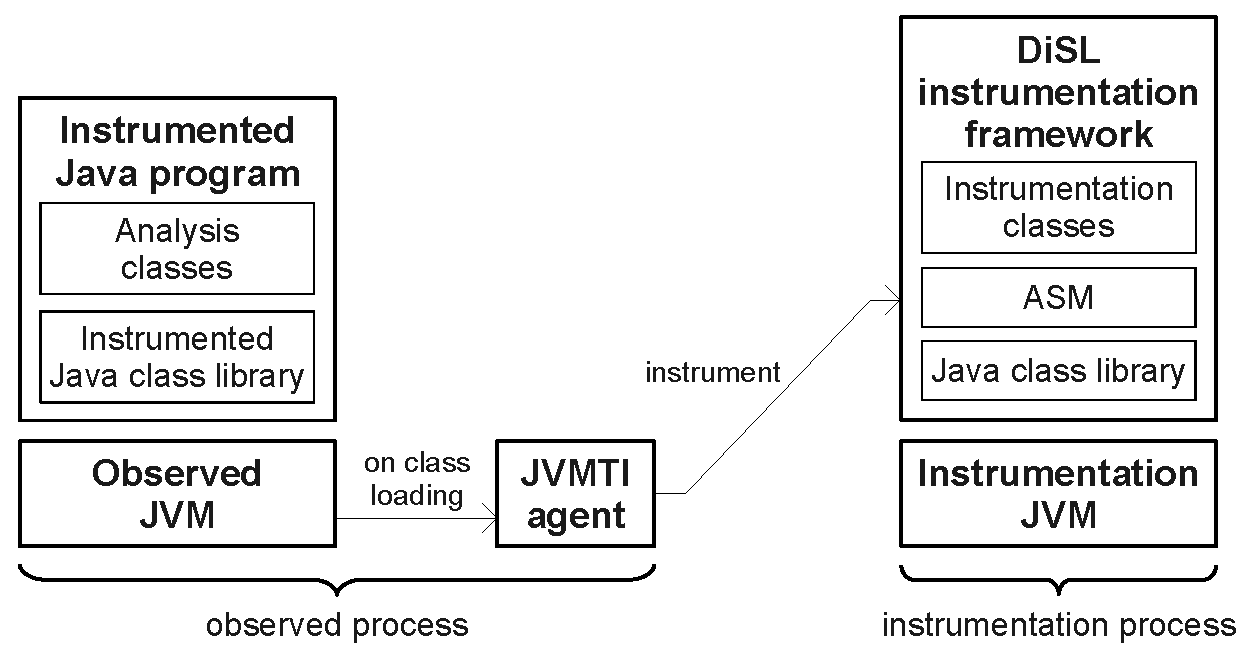
\includegraphics[width=0.95\textwidth]{fig/architecture}
\caption{Architecture of DiSL.}\label{fig:arch}
\end{figure}


To minimize perturbation in the observed program, DiSL performs bytecode instrumentation within a separate Java Virtual Machine (JVM) process, that is, the \mbox{\emph{instrumentation process}}.
In this way, class loading and initialization triggered by the instrumentation framework do not happen within the \mbox{\emph{observed process}}.

As illustrated in Figure~\ref{fig:arch}, a native JVMTI agent\footnote{\url{http://download.oracle.com/javase/6/docs/platform/jvmti/jvmti.html}} captures all class loading events (starting with \code{java.lang.Object}) in the observed JVM and sends every class as a byte array to the DiSL instrumentation framework through a socket.
Here, DiSL uses ASM for instrumentation.

\begin{figure}
\centering
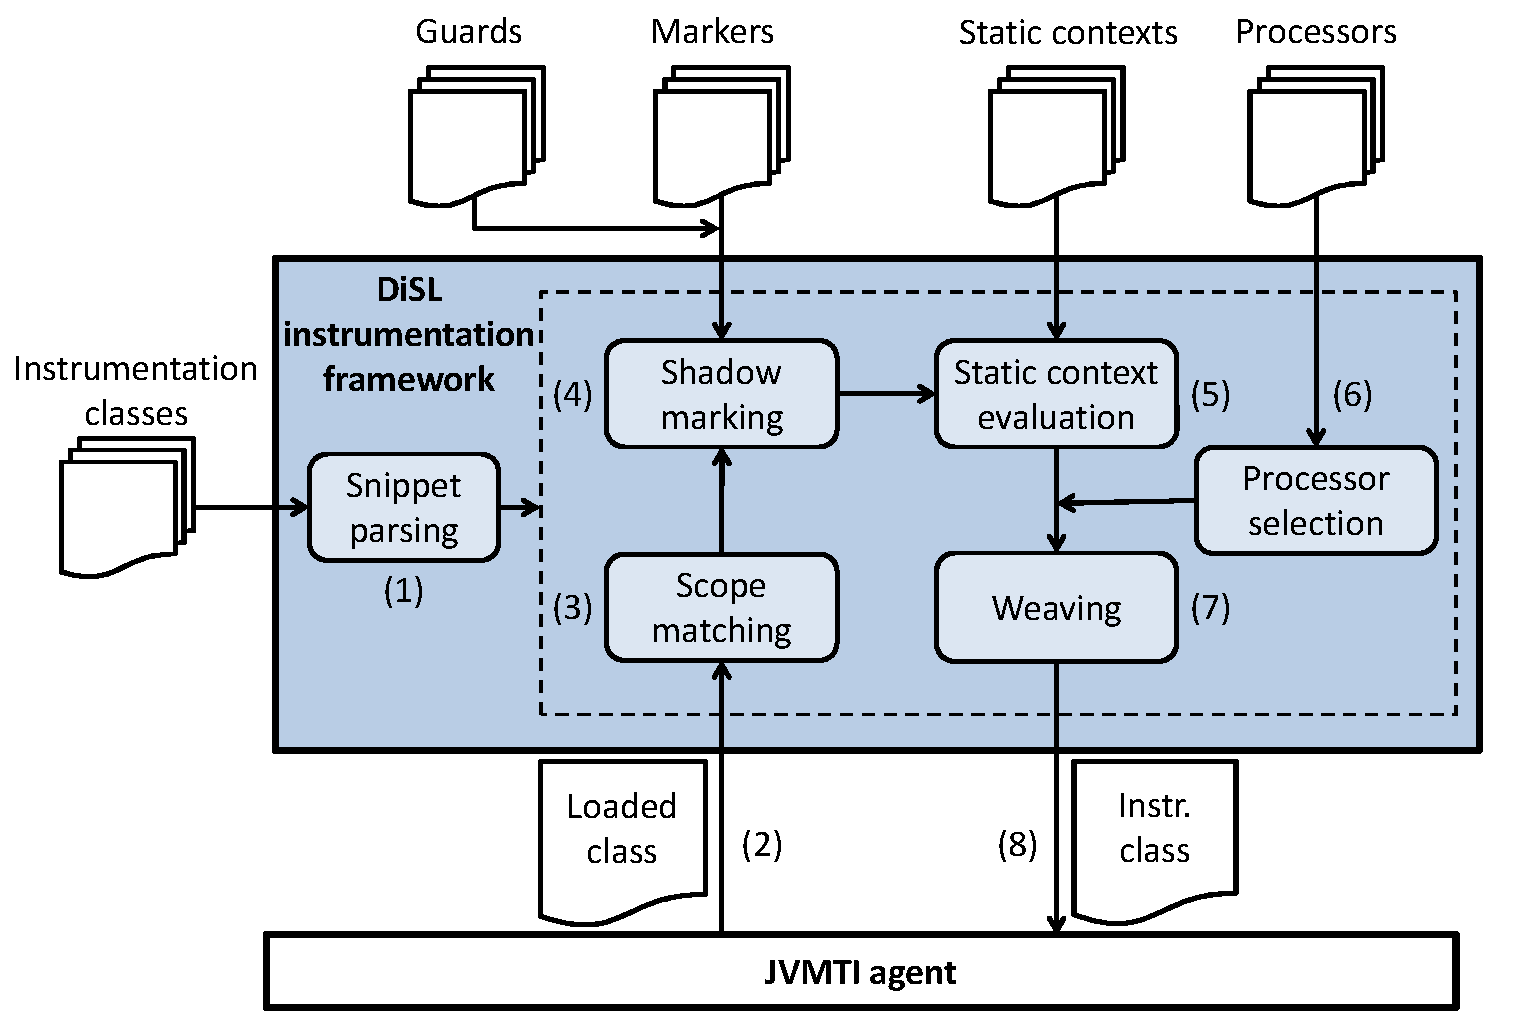
\includegraphics[width=0.90\textwidth]{fig/overview}
\caption{Overview of the DiSL instrumentation process.}\label{fig:overview}
\end{figure}

Figure~\ref{fig:overview} gives an overview of the DiSL instrumentation process.
During initialization, DiSL parses all instrumentation classes (step~1).
Then it creates an internal representation for snippets and initializes the used markers, guards, static contexts, and argument processors.
When DiSL receives a class from the JVMTI agent (step~2), the instrumentation process starts with the snippet selection.
The selection is done in three phases, starting with scope matching (step~3).
Then, bytecode regions are marked using the markers associated with the snippets selected in the previous phase. %scope matching phase.
Finally, marked bytecode regions are evaluated by guards and only snippets with at least one valid marked region are selected (step~4).

At this point, all snippets that will be used for instrumentation are known.
Static contexts are used to compute the static information required by snippets (step~5).
As described in Section~\ref{sec:Advanced}, custom static contexts allow programmers to declare expressions to be evaluated at instrumentation time.
However, if such expressions do not require custom context information, they can simply be embedded in the snippet code.

Argument processors are evaluated for snippets, and argument processor methods that match method arguments are selected (step~6).
All the collected information is finally used for instrumentation (step~7).
Argument processors are applied, and calls to static contexts are replaced with the computed static information.
The framework also generates the bytecodes to access dynamic context information.
To prevent the instrumentation code from throwing exceptions that could modify the control flow in the observed program, DiSL automatically inserts code intercepting all exceptions originating from the snippets, reporting an error if an exception is thrown (and not handled) by the instrumentation.
Finally, the instrumented class is returned to the observed JVM (step~8) where it is linked.

\section{Acknowledgments}\label{sec:Acks}

The initial version of this tutorial has been based on a paper by Lukáš Marek, Yudi Zheng, Danilo Ansaloni, Lubomír Bulej, Aibek Sarimbekov, Walter Binder and Petr Tůma.

\newpage
\appendix

\section{Running DiSL}\label{sec:Setup}

This appendix provides a step-by-step guide to download, compile, and run the DiSL framework.
The current release of DiSL is tested with Java 7 and Linux, for which we provide scripts to compile and run the framework.
To build DiSL and the examples, Java 7 JDK must be installed on the system,
including rudimentary tools such as \code{ant}, \code{gcc}, \code{make} and \code{python}.

% The section describes step-by-step guide how to invoke analysed (instrumented) application under DiSL.
% The guide uses the basic example included directly with DiSL sources, but it is recommended to use similar structure and starting scripts in all DiSL projects.

The source code of DiSL can be downloaded from the DiSL home page\footnote{\url{http://disl.ow2.org}}, hosted by the OW2 Consortium.
In particular, DiSL releases are available at \url{http://forge.ow2.org/projects/disl/files/}.
After downloading and extracting the latest release candidate of DiSL, the main directory contains a \code{README} file that describes how to compile the framework and access additional documentation.\footnote{\url{http://disl.projects.ow2.org/xwiki/bin/view/Main/Doc/}}

\medskip
A very simple example of a DiSL instrumentation can be found in the \code{example/smoke} directory.
In this example the observed program (i.e., \code{example/smoke/app/src/Main.java}) prints a hello-world message, while the instrumentation (i.e., \code{example/smoke/instr/src/DiSLClass.java}) inlines the code to print a message at the beginning and at the end of the main method body.

Listing~\ref{lst:example-commands} shows the sequence of commands needed to compile the DiSL framework and to run the example.
In line~\ref{src:compile1}, we compile the DiSL framework.
Line~\ref{src:run} runs the example program.

\begin{lstlisting}[
caption={Compiling the framework and running the included DiSL example.},
label={lst:example-commands},
language=c,numbers=left,escapeinside={@}{@},
]
[disl]@\$@ ant @\label{src:compile1}@
[disl]@\$@ cd example/app/smoke @\label{src:chdir1}@
[disl/example/app/smoke]@\$@ ant run @\label{src:run}@
\end{lstlisting}


\medskip
Listing~\ref{lst:example-output} shows the expected output of the instrumented program.
Line~\ref{src:baseprogram} is the message printed by the observed program, while lines~\ref{src:instr1} and~\ref{src:instr2} are the messages printed by the instrumentation.

\begin{lstlisting}[
caption={Output of the included DiSL example.},
label={lst:example-output},
language=c,numbers=left,escapeinside={@}{@},
]
Instrumentation: Before method main @\label{src:instr1}@
Application: Inside method main @\label{src:baseprogram}@
Instrumentation: After method main @\label{src:instr2}@
\end{lstlisting}


\medskip
It is possible to use the \code{disl.py} script to invoke DiSL with user-defined instrumentations, provided the following rules are adhered to:
\begin{itemize}
\item All the instrumentation and the analysis classes must be packed into a single jar~file, including any external libraries used by the analysis.
Such libraries can be added to the jar~file using, for example, the \code{jarjar}\footnote{\url{http://code.google.com/p/jarjar/}} tool.

\item The \code{MANIFEST.MF} file in the \code{META-INF} directory of the jar~file must list all the DiSL classes used for the instrumentation; Listing~\ref{lst:example-manifest} shows the manifest file of the included example.
In this case, the instrumentation consists of a single class (i.e., \code{DiSLClass}) that can be found in the default package.
\end{itemize}

Run \code{disl.py -h} for info how to use the script and to list all available parameters.

\begin{lstlisting}[
caption={Manifest file of the included DiSL example.},
label={lst:example-manifest},
language=c,escapeinside={@}{@},
]
Manifest-Version: 1.0
DiSL-Classes: DiSLClass
\end{lstlisting}


\medskip
An archive of all examples and tools presented in this paper can be downloaded from the DiSL release page.
This archive must be extracted within the main directory of DiSL and includes an additional \code{README} file that describes how to run the examples.
Listing~\ref{lst:examples} shows how the \code{runExample.sh} script can be used to run the example shown in Figure~\ref{fig:instr-prof-simple-prof} of this paper.

\begin{lstlisting}[
caption={Running the profiler example presented in Figure~\ref{fig:instr-prof-simple-prof}.},
label={lst:examples},
language=bash,escapeinside={@}{@},
]
[disl/examples]@\$@ ./runExample.sh \
2.1-Method_Execution_Time_Profiler-Figure_1
\end{lstlisting}

\newpage

\section{JVM Crashes}\label{sec:Crashes}

DiSL is designed to instrument application together with whole Java Class Library.
It uses custom java agent implemented in C to intercept loading of every class.
A class is instrumented before it is loaded by the JVM, thus the application always uses instrumented version of the class.
Thanks to such a mechanism, DiSL is able to instrument even core classes like java.lang.Object.
This however has unfortunate consequences.

Current versions of Oracle JVM are not able to handle bigger modifications to classes loaded during the initial stage of the JVM startup.
Sadly, instead of producing some meaningful error message, the JVM crashes instantly.

The solution is to ether modify the instrumentation or exclude from instrumentation a class (method) that caused the problem.
As pointing to the specific class often requires a lot of effort, we recommend to exclude all the core classes during development and seek the solution during testing (deployment).

Here, we describe possible solutions for the crashing problem.

\subsection{Exclusion using scopes}

First method is to instrument only a part of an application.
This is possible using scope parameter of an annotation.

\begin{lstlisting}[
caption={Instrumenting only part of an application using scope},
label={lst:cscope},
language=java,escapeinside={@}{@},
]
@Before(marker=BodyMarker.class, scope="Main.*")
\end{lstlisting}

Scope in Listing~\ref{lst:cscope} restricts instrumentation only to all methods an a Main class (in any package).
The Scope ensures that none of the bootstrap classes is instrumented which resolves the problem.

\subsection{Exclusion using exclusion lists}


Another option is to use exclusion list.
Exclusion list contains set of classes excluded from instrumentation.
Passing of exclusion list to the instrumentation is done via \code{-s\_exclusionlist} parameter of the \code{disl.py} startup script.

Listing~\ref{lst:clist} enumerates all expression used to exclude most of the classes from Java class library.
It is recommended, that during the development, the exclusion list should include classes that are not testing the core functionality and refine it to the level of exclusion of a particular methods during deployment.

\begin{lstlisting}[
caption={Exclusion list excluding most of the classes of Java Class Library},
label={lst:clist},
language=bash,escapeinside={@}{@},
]
# RECOMMENDED TO BE EXCLUDED
sun.instrument.*.*
java.lang.Object.*
java.lang.Thread.*
ch.usi.dag.disl.*.*

# EXCLUDES MOST OF THE JDK CLASSES
org.jcp.*
org.omg.*
org.xml.*
org.ietf.*
java.*.*
javax.*.*
com.sun.*
com.apple.*
sun.*.*
sunx.*
\end{lstlisting}

Note that expressions in the exclusion list is using the same expression language as the Scope pattern.
Precise description of the scoping language is present in Javadoc (see ScopeImpl class).

\end{document}
